%!TEX root = ../../csuthesis_main.tex
\chapter{绪论}

\section{研究背景及意义}
随着人类社会与科技的飞速发展,对广袤海洋的认知、开发与利用已成为衡量国家综合国力的重要标志,并以前所未有的速度向深远海拓展。海洋不仅是地球上最大的资源宝库,蕴藏着丰富的生物、矿产(石油、天然气、可燃冰、多金属结核等)和可再生能源,更是关乎全球气候、生态平衡和国家战略安全的关键领域。在提出“海洋强国”的当下,高效、可靠的水下交通、运输、探测与作业能力成为关键支撑。

特别是对于蕴藏着丰富战略资源的深海区域,实现有效抵达和精细作业是进行科学考察、资源勘探、环境监测以及海底设施(如管线、电缆、观测网)布放与维护等活动的前提。传统的载人潜水器虽然能够执行部分任务,但面临着生命支持系统复杂、作业时间受限、以及对潜航员生理和心理的巨大考验等问题,尤其是在高压、黑暗、低温的极端深海环境中,其风险和成本居高不下。因此,发展和应用能够替代或辅助人类在水下执行复杂任务的无人化装备,已成为国际海洋工程技术发展的重要趋势。

由水下机器人承载起的水下交通对于深海的探测工作具有重要意义。广袤的海洋,尤其是深远海,人类难以直接进入。水下运载平台的运输能力,使得搭载着探测传感器的系统能够克服水深、压力、黑暗等障碍,抵达遥远、未知或危险的水下区域。水下平台的机动性、多传感器的感知能力、自适应控制的导航和避障能力,使其能够按照预定路径或自适应路径进行移动,对大面积海域或海底进行系统性的扫描和测绘,如海底地形地貌勘测、管线巡检、资源普查等,丰富了探测范围与探测能力。\cite{CaiWeiZiZhuShuiXiaJiQiRenHaiDiReYeQuYingYongZongShu2023}

为了克服水下环境的限制,各类水下机器人应运而生,主要包括遥控水下机器人(Remotely Operated Vehicle, ROV)和自主水下机器人(Autonomous Underwater Vehicle, AUV)。ROV通过线缆与母船连接,由操作员远程控制,具有实时监控、精确操作和强作业能力的优点,广泛应用于海底观测、资源勘探、管线检查、水下结构物安装与维护、沉船打捞、水产养殖等领域。随着水下任务复杂度的提升,特别是涉及物品搬运、设备部署、样品采集与回收等需求的增加,对具备水下运输能力的ROV提出了更高的要求。

水下遥控运载机器人(Remotely Operated Vehicle, ROV),作为一种通过脐带缆从母船获取动力和传输控制/数据信号的无人潜水器,能够搭载多种传感器和作业工具,凭借其操作灵活、作业时间长、环境适应性强等优势,在这一需求下应运而生并扮演着越来越重要的角色。ROV在水下运动时,其动力学行为受到自身结构、流体介质以及所携带载荷的复杂耦合影响,包括非线性的水动力(流体阻力、附加质量效应等)、科里奥利力、重力与浮力变化、推进器推力特性以及环境干扰(如洋流)等。当ROV携带不同形状、尺寸和质量的载荷时,其整体的惯性特性和水动力特性会发生显著变化,这使得建立一个能够精确描述其运动行为的动力学模型成为一大难题。

更为关键的是,模型中的许多核心参数,特别是描述流体与机器人相互作用的“水动力系数”(如阻尼系数、附加质量系数),往往难以通过纯理论计算精确获得,且可能随工作状态和环境变化而改变。因此,仅仅建立理论模型是不够的,必须通过有效的方法对这些关键参数进行动态辨识。通过分析ROV实际运行(或高保真仿真)过程中的运动状态数据,包括导航轨迹、速度、加速度等,结合参数辨识算法,实时反推出准确的水动力系数,才能获得真正贴合实际工况的高精度动力学模型。这对于后续设计能够适应载荷变化和环境扰动的高性能控制器至关重要。

在拥有了经过辨识校准的精确动力学模型之后,需要实现一个高保真的仿真平台和控制器,通过机器人跟踪预设路径的实际效果以验证动力学模型的辨识表现。在物理样机制造和昂贵的水池试验之前,高保真仿真平台可以对ROV的机械结构、推进器配置、传感器布局等设计方案进行快速迭代和评估,能够测试和验证导航、制导与控制(NGC)算法,以及图像处理、路径规划等上层智能算法,而无需担心损坏真实ROV或应对复杂的实际测试准备。此外,高保真仿真平台可以轻易地改变水动力参数、质量分布等,可以研究这些参数对ROV运动性能的影响,加深对ROV动力学特性的理解。

综上所述,用于水下运输的遥控运载机器人的建模和仿真,旨在深化对载荷变化下水下机器人复杂动力学行为的理解,探索将先进优化算法应用于水动力参数动态辨识的有效途径,并深入研究模型预测控制在解决此类强非线性、多约束、时变系统高精度轨迹跟踪问题上的应用潜力与理论方法。有望显著提升水下运输机器人的轨迹跟踪精度、作业稳定性以及对变化的载荷与环境的适应能力,为“海洋强国”战略的实施提供关键技术支撑和人才储备。

\section{水下机器人分类}

常见的水下机器人可根据其外形结构、工作情景与应用范围分为三类:遥控式水下机器人,载人潜水器,自治水下机器人。

遥控潜水器 (Remotely Operated Vehicle,简称ROV) 是一种无人水下机器人,其携带有一根长电缆,通过这根电缆传送能源和信号。操作者可以通过这根电缆对机器人进行遥控操作。ROV的优点是能够在一个小范围内精细的观测,可以携带机械手和作业工具在海底进行精细取样作业,比如采集岩石、海底沉积物,收集失落在海底的物体,取水样、泥样等。

载人潜水器(Human Occupied Vehicle,简称 HOV),是一种可以携带研究人员的大型水下航行器。HOV 可由内部潜水器内部的研究人员进行操纵,具有较强的水下作业能力。HOV 不是完全自主运动的,需要母船进行氧气以及能源的补给,因此航程一般较短。

自治水下机器人(Autonomous Underwater Vehicle,简称 AUV),是一种完全自主的无人式水下机器人。AUV 在下水之前就已经被写入相关控制程序,可以按照预先设置好的控制策略进行自主航行,具有较高的智能水平。

\section{国内外研究现状}
\subsection{ROV建模与仿真技术研究现状}
水下机器人动力学建模是利用物理学原理,来建立描述机器人运动状态,如位置、姿态、速度和加速度)与其所受各种力及力矩之间关系的数学模型。建立水下机器人动力学模型的核心目标是深入理解机器人在复杂水下环境中的行为规律,并能够预测其在不同驱动力和环境干扰下的运动响应。建立精确的动力学模型对于后续的控制系统设计至关重要,因为它为控制器提供了计算所需驱动力以实现期望运动的基础。同时,该模型也是进行仿真测试、验证算法、优化机器人设计以及辅助导航状态估计的关键工具。在建模过程中,需要综合考虑机器人的刚体惯性效应、复杂的水动力效应、静水恢复力、推进系统的推力特性,以及来自水流、波浪或缆绳等外部环境的干扰力。最终,动力学模型通常表现为一套耦合的、非线性的六自由度(6-DOF)常微分方程组,它系统地刻画了水下机器人在力和力矩作用下的完整动态响应特性。

近几十年来,世界各地的研究人员针对ROV动力学建模进行大量研究工作,许多经典的动力学建模方法被工程应用。现阶段使用较多的动力学建模方法是将ROV视为刚体,对ROV进行受力分析,从而通过刚体动力学理论建立动力学模型。国内李殿璞学者\cite{LiDianPuChuanBoYunDongYuJianMo2008}用牛顿-欧拉法推导了水下航行器动力学模型的一般表达式,将水下航行器的动力学分解为水平面水动力与垂直面水动力,分别推导表达式;挪威学者Fossen系统地提出了ROV的流体动力学模型\cite{fossenHandbookMarineCraft2021},现该模型已经被广泛使用在ROV运动控制领域,成为该领域内的标准模型;我国孙元泉、马运义等人\cite{2001潜艇和深潜器的现代操纵理论与应用}也对水下航行器进行建模研究,将水下航行器建模进一步划分为垂直面操纵模型和水平面操纵模型;Malte von Benzon等\cite{vonbenzonOpenSourceBenchmarkSimulator2022}在Fossen模型的基础上,使用集中质量法对连接ROV和顶部设施的系绳进行了建模,并将其作为ROV模型的力输入。

在建立 AUV 的理论模型之后,不同几何特征与应用场景的 AUV 需要通过实验方法进行计算获得具体的模型参数。水下航行器由于其处于非结构性环境下,水域情况复杂,难以用简单的数学公式精确描述,环境干扰对系统影响大,无法求得动力学模型参数的解析解。除此之外,ROV为了搭载各种传感器和作业工具,外形通常不是理想的流线型,这导致了复杂的流场环境,使得水动力特性更加难以求解。

有许多学者水动力参数的辨识方法进行研究,对于水动力参数辨识的方法主要分为:实验数据驱动法、模型拟合法、数值计算法(CFD)。在实验数据驱动法中,Massimo Caccia\cite{cacciaModelingIdentificationOpenframe2000}通过收集传感器数据,利用最小二乘法先后辨识了阻力和推进器安装系数与系统惯性矩阵;Eschmann等\cite{eschmannDataDrivenSystemIdentification2024}利用机体传感器数据辨识四旋翼飞行器的惯性参数、推力曲线、力矩系数和一阶电机延迟,以此完善飞行器动力学模型,该方法可以被借鉴到水下机器人的辨识过程中;Deng等人\cite{dengIdentificationAutonomousUnderwater2021}比较了无迹卡尔曼滤波、扩展卡尔曼滤波和时域离散优化卡尔曼滤波器三种滤波算法在辨识水动力参数上的准确性,提出了自回归滑动平均( ARMA )噪声模型以提高估计精度和扰动抑制性能。模型拟合法提供了一种数据驱动的方法,可以直接从ROV的实际运动数据中提取这些关键参数,其中,Zohedi\cite{zohediSYSTEMIDENTIFICATIONSI2023}、Aras\cite{arasThrusterModellingUnderwater2013}等采用MATLAB Simulink的系统辨识工具箱,选择合适的模型拟合ROV系统运动轨迹,用于控制ROV悬浮状态的稳定性。数值计算法中,Zhang\cite{zhangStudyImpactProcess2017}、Zheng\cite{zhengStudyHydrodynamicPerformance2017}等人利用计算流体动力学的方式,利用商业软件GAMBIT或FLUENT建立网格和划分流域,对不同工况结果进行仿真求解,获得水动力系数较为容易,但其求解结果十分依赖于网格设置精度。

\subsection{ROV仿真平台研究现状}

随着技术的发展,仿真平台技术突飞猛进,被广泛使用在ROV的研发过程中。水下机器人仿真平台是一种利用数字化技术实现水下环境与机器人的虚拟再现的重要工具,能够有效支持算法开发、任务规划及环境感知等多方面的研究与实践\cite{cookSurveyAUVRobot2014}。其核心目的是通过虚拟环境代替真实场景进行实验和测试,以降低实验风险和成本,同时提高算法开发效率和仿真结果的可控性。当前主要的ROV仿真平台如下:

\subsubsection{Gazebo}

Gazebo 是一款功能强大的开源 3D 物理仿真引擎,在机器人学研究和开发中得到了广泛应用。其可以与机器人操作系统(ROS)结合,支持通过特定插件包进行扩展,实现各项高保真仿真功能,主要包括:1)动力学仿真:Gazebo 支持多种高性能的物理引擎,如 ODE、SimBody、ART、Bullet 等。用户可以在机器人模型三维模型文件的基础上设置机器人及周围环境的物理;2)可视化三维流体环境:用户可以创建或导入复杂的海底地形、水下结构物(如管道、沉船、平台)、珊瑚礁等三维模型,构建逼真的水下作业场景;3)流体仿真:引入流体动力学模型,模拟水下机器人在流体中的运动响应;4)视觉开发:模拟水下光学图像,可以调整水体浑浊度、光照等参数,用于视觉导航、目标识别算法的开发。

\subsubsection{DAVE}

DAVE是一个构建水下机器人仿真环境的开源功能包。DAVE 的核心设计理念是高度模块化。它旨在提供一个框架,用户可以像搭积木一样组合不同的软件模块来快速构建和仿真各种类型的水下航行器及其任务。除此之外,DAVE 提供了丰富的用于实现机器人行为和任务逻辑的框架,包括航向保持、深度保持、速度保持、航点跟踪,其允许用户定义一系列任务或目标,并让机器人自主执行。更侧重于水下机器人自主行为的模块化设计、任务级控制和决策逻辑的快速原型验证。它的物理仿真和渲染可能不如Gazebo精细,但其组件化架构在构建和测试复杂自主系统方面有优势。

\subsubsection{MATLAB/Simulink}

MATLAB/Simulink 是工程领域广泛使用的数学计算和基于模型的设计环境,在水下机器人仿真中也扮演着非常重要的角色。它们提供了一套强大而灵活的工具,用于水下机器人的建模、控制系统设计、算法开发和仿真分析。MATLAB/Simulink 提供了多种控制系统设计工具箱,支持设计和调试PID控制器,并进行参数整定;设计和仿真MPC控制器,能够处理约束和优化性能指标。但其物理真实感和3D渲染比不上专业物理仿真引擎;对于复杂的水下环境的模拟能力有限,对于模拟传感器的物理感知过程较为粗糙。

\subsection{ROV运动控制技术研究现状}

水下机器人的控制器设计与轨迹跟踪是实现其自主或遥控作业能力的核心环节,确保机器人能够精确、稳定地按照预定的路径或指令运动。控制器根据机器人的当前状态与期望状态之间的误差,计算出需要施加给推进器系统的控制指令。这个过程必须克服水下环境带来的巨大挑战,包括机器人自身复杂的非线性、强耦合动力学特性,难以精确建模的水动力参数及其时变性,以及无处不在的外部干扰,如未知的水流、波浪影响等。轨迹跟踪要求控制器不仅要使机器人到达某个点,更要使其在运动过程中紧密地、平滑地跟随一条在空间和时间上都已定义好的路径。为了实现有效的轨迹跟踪,研究人员开发了多种控制策略。

\subsubsection{PID控制}

PID(Proportional-Integral-Derivative,比例-积分-微分)控制器是一种在工业控制应用中常见的反馈控制器。它的核心思想是根据被控对象的期望值与实际输出值之间的误差,通过比例、积分、微分三种运算的线性组合来产生控制信号,驱动执行机构,从而使实际输出值趋近期望值。简单的PID(比例-积分-微分)\cite{liuUnderwaterRemotelyOperated2023}控制因其结构简单、易于实现而被广泛应用\cite{zohediSYSTEMIDENTIFICATIONSI2023},但在面对强非线性和显著不确定性时往往性能受限,需要对PID控制进行改进或者与其他控制策略复合控制,包括神经网络自回归PID控制\cite{hernandez-alvaradoNeuralNetworkBasedSelfTuning2016},模糊PID控制\cite{dongDepthControlROV2020a},结合改进粒子群优化算法PID控制\cite{liuUnderwaterRemotelyOperated2023a}。

\subsubsection{滑模控制}

滑模控制是一种非线性鲁棒控制方法,其核心思想是将系统的控制问题分解为两个阶段,在到达阶段上,需要设计一个控制律,使得系统的状态轨迹能够在有限时间内到达并保持在一个预先设计好的切换超曲面上,这个超曲面也称为滑模面; 一旦系统状态轨迹到达滑模面上,控制律将迫使状态轨迹沿着该滑模面滑动,进入滑动阶段,并最终趋向于平衡点,滑模控制因其对模型不确定性和外部干扰的强鲁棒性而被广泛应用于水下机器人领域\cite{renROVSlidingMode2023},Chen等\cite{chenFunctionbasedRobustSliding2025}将滑膜控制与干扰观测器相结合,用于解决ROV抖振与动力学模型不确定性问题;Bessa等\cite{bessaDepthControlRemotely2008}通过自适应模糊算法与滑膜控制算法相结合来增强不确定性干扰补偿,在保证消除抖振的同时实现了光滑的曲线跟踪。

\subsubsection{基于智能算法的自适应控制}

随着计算机技术和人工智能的发展,智能算法,如神经网络、模糊逻辑、遗传算法、粒子群优化、强化学习等被越来越多地引入到自适应控制领域,形成了基于智能算法的自适应控制。这种结合被认为是控制领域的一个先进发展方向,因为它能够克服传统自适应控制的一些局限性,并为处理更复杂、更不确定的系统提供了新的思路和工具。Bagheri等\cite{bagheriTrackingPerformanceControl2010}利用自适应神经网络控制有效提升了水下机器人的轨迹跟踪性能;Chu等\cite{chuObserverBasedAdaptiveNeural2017}提出了基于局部RNN的自适应终端滑模状态观测器,以保证轨迹跟踪误差在有限时间内得以收敛,提高了轨迹跟踪的精度和稳定性。

\subsubsection{模型预测控制(MPC)}

模型预测控制(MPC)将ROV的动力学模型纳入控制流程中,该方法利用已建立的、尽可能精确的ROV动力学模型预测系统在未来一段时间内对一系列候选控制输入序列的响应。基于这些预测结果,MPC通过求解一个在线优化问题,寻找能够在预测时域内最小化预定性能指标并同时满足各种物理约束的最优控制输入序列,相比那些不直接进行基于模型预测优化的控制器,往往能实现更优的控制性能和对未来行为的主动管理。Shen等\cite{shenTrajectoryTrackingControl2018}提出基于李雅普诺夫的模型预测控制器,优化了闭环控制系统的稳定性;Hu等\cite{huDisturbanceObserverBasedModel2024}将扩张主动观测器与模型预测控制相结合,用于处理ROV的外部信号干扰和模型噪音,有效屏蔽了外部不可预测的干扰信号;Hu等将MPC控制与扩展主动状态观测器相结合,与传统的干扰观测器相比,所开发的算法具有同时处理外部干扰和系统测量噪声的能力。

\section{论文组织结构}

本文主要研究了用于水下运输的遥控运载机器人的建模与仿真,首先对水下机器人进行运动学建模和动力学建模,建立ROV运动控制的基础理论,然后提出了基于最小二乘法和扩展卡尔曼滤波器的动力学参数辨识算法,最后通过UUV Simulator仿真系统完成了对ROV运动控制的仿真,并且比较两种算法辨识结果在轨迹跟踪这一任务需求上的优劣。

本文研究内容及分布如图\ref{f.thesis_framework}所示。

\begin{figure}[hbt]
    \centering
    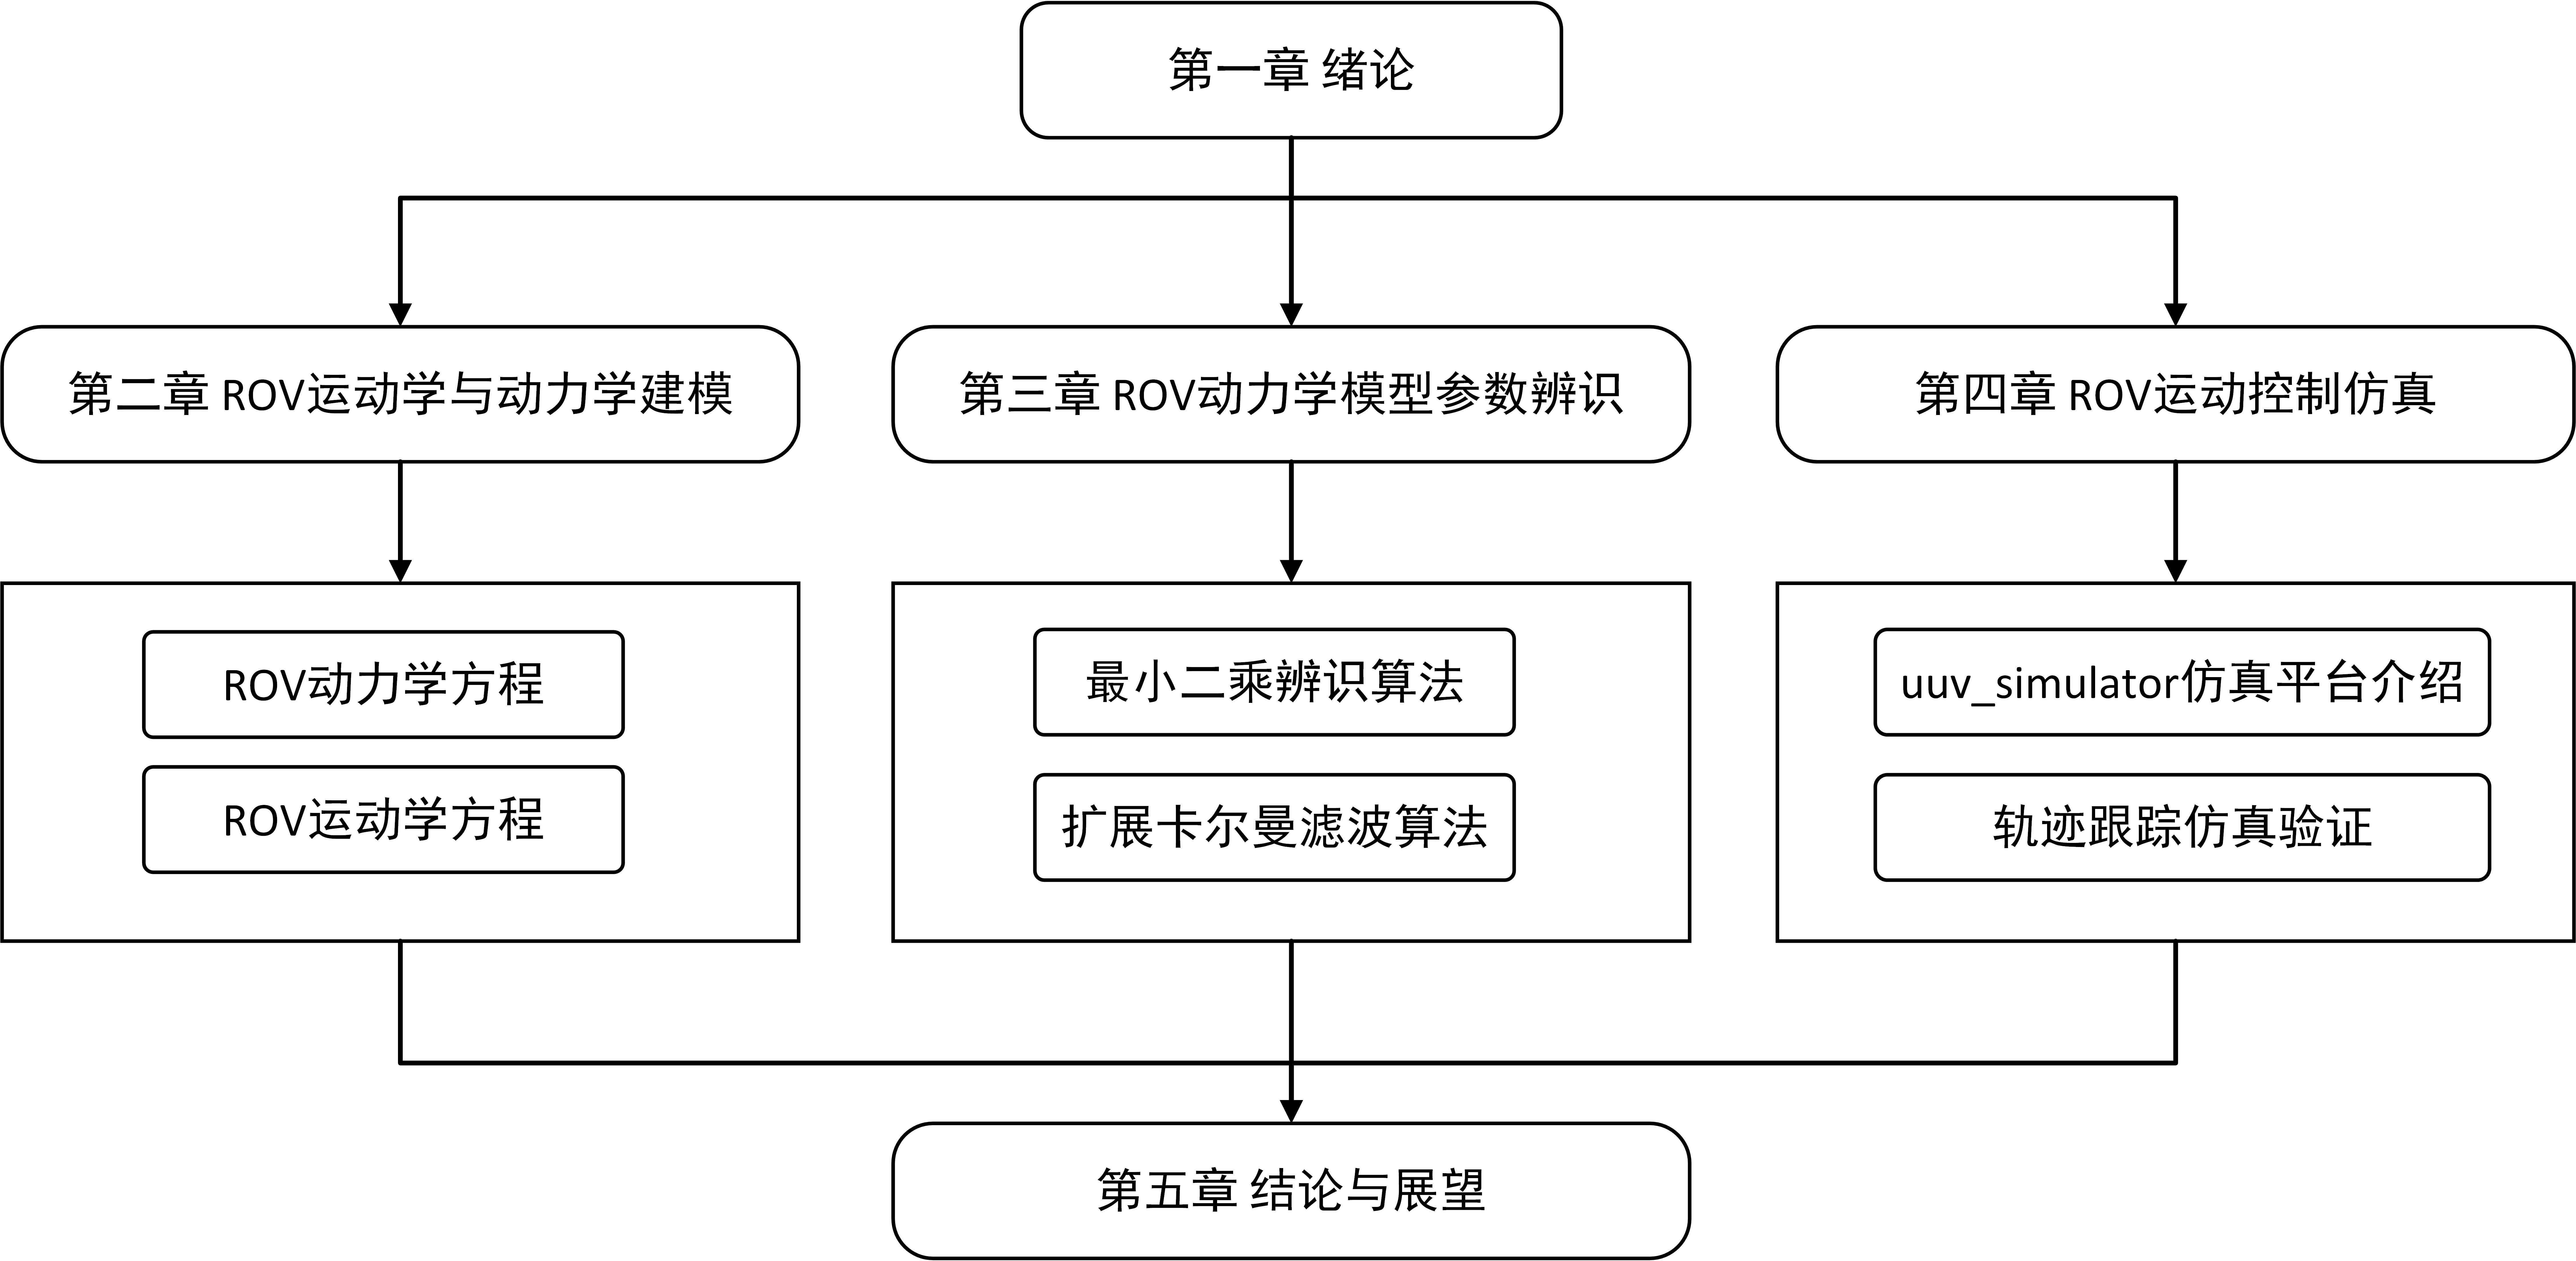
\includegraphics[width=\linewidth]{images/chapter1/论文架构图.png}
    \caption{本文研究结构}
    \label{f.thesis_framework}
\end{figure}

第一章主要介绍了研究课题的背景和意义,介绍了本文研究对象ROV建模与仿真技术、ROV水下运动控制技术在当下国内外的发展现状,并简要阐述了本文的主要研究内容。

第二章主要完成了ROV运动学模型与动力学模型的建立,ROV运动学模型与动力学模型是控制ROV运动的基础。在本章,首先介绍了Bluerov2的主体结构与组成,通过建立相关坐标系、定义相关运动参数以获得ROV运动学方程;通过建立水动力阻尼模型,对ROV进行受力分析,得到ROV的动力学方程。

第三章主要介绍了最小二乘算法与扩展卡尔曼滤波器算法的原理,分别利用其辨识动力学模型的未知参数,完成了动力学模型参数辨识的算法设计,通过MATLAB/Simulink仿真实现了扩展卡尔曼滤波器的参数辨识过程。

第四章主要介绍了UUV Simulator的主要架构,ROV控制器设计,在仿真平台上控制ROV按照预设轨迹运动,并通过修改仿真平台中ROV动力学模型参数,比较最小二乘算法与扩展卡尔曼滤波器算法的辨识效果在轨迹跟踪这一任务上的实际表现,完成了对Bluerov2的轨迹跟踪控制功能。

第五章主要对本文工作进行总结,并对本课题以后的研究方向进行展望。

\newpage